\documentclass{standalone}
\usepackage{tikz}
\usetikzlibrary{patterns, positioning}
\usepackage[sfdefault]{ClearSans} %% option 'sfdefault' activates Clear Sans as the default text font
\usepackage[T1]{fontenc}

\begin{document}
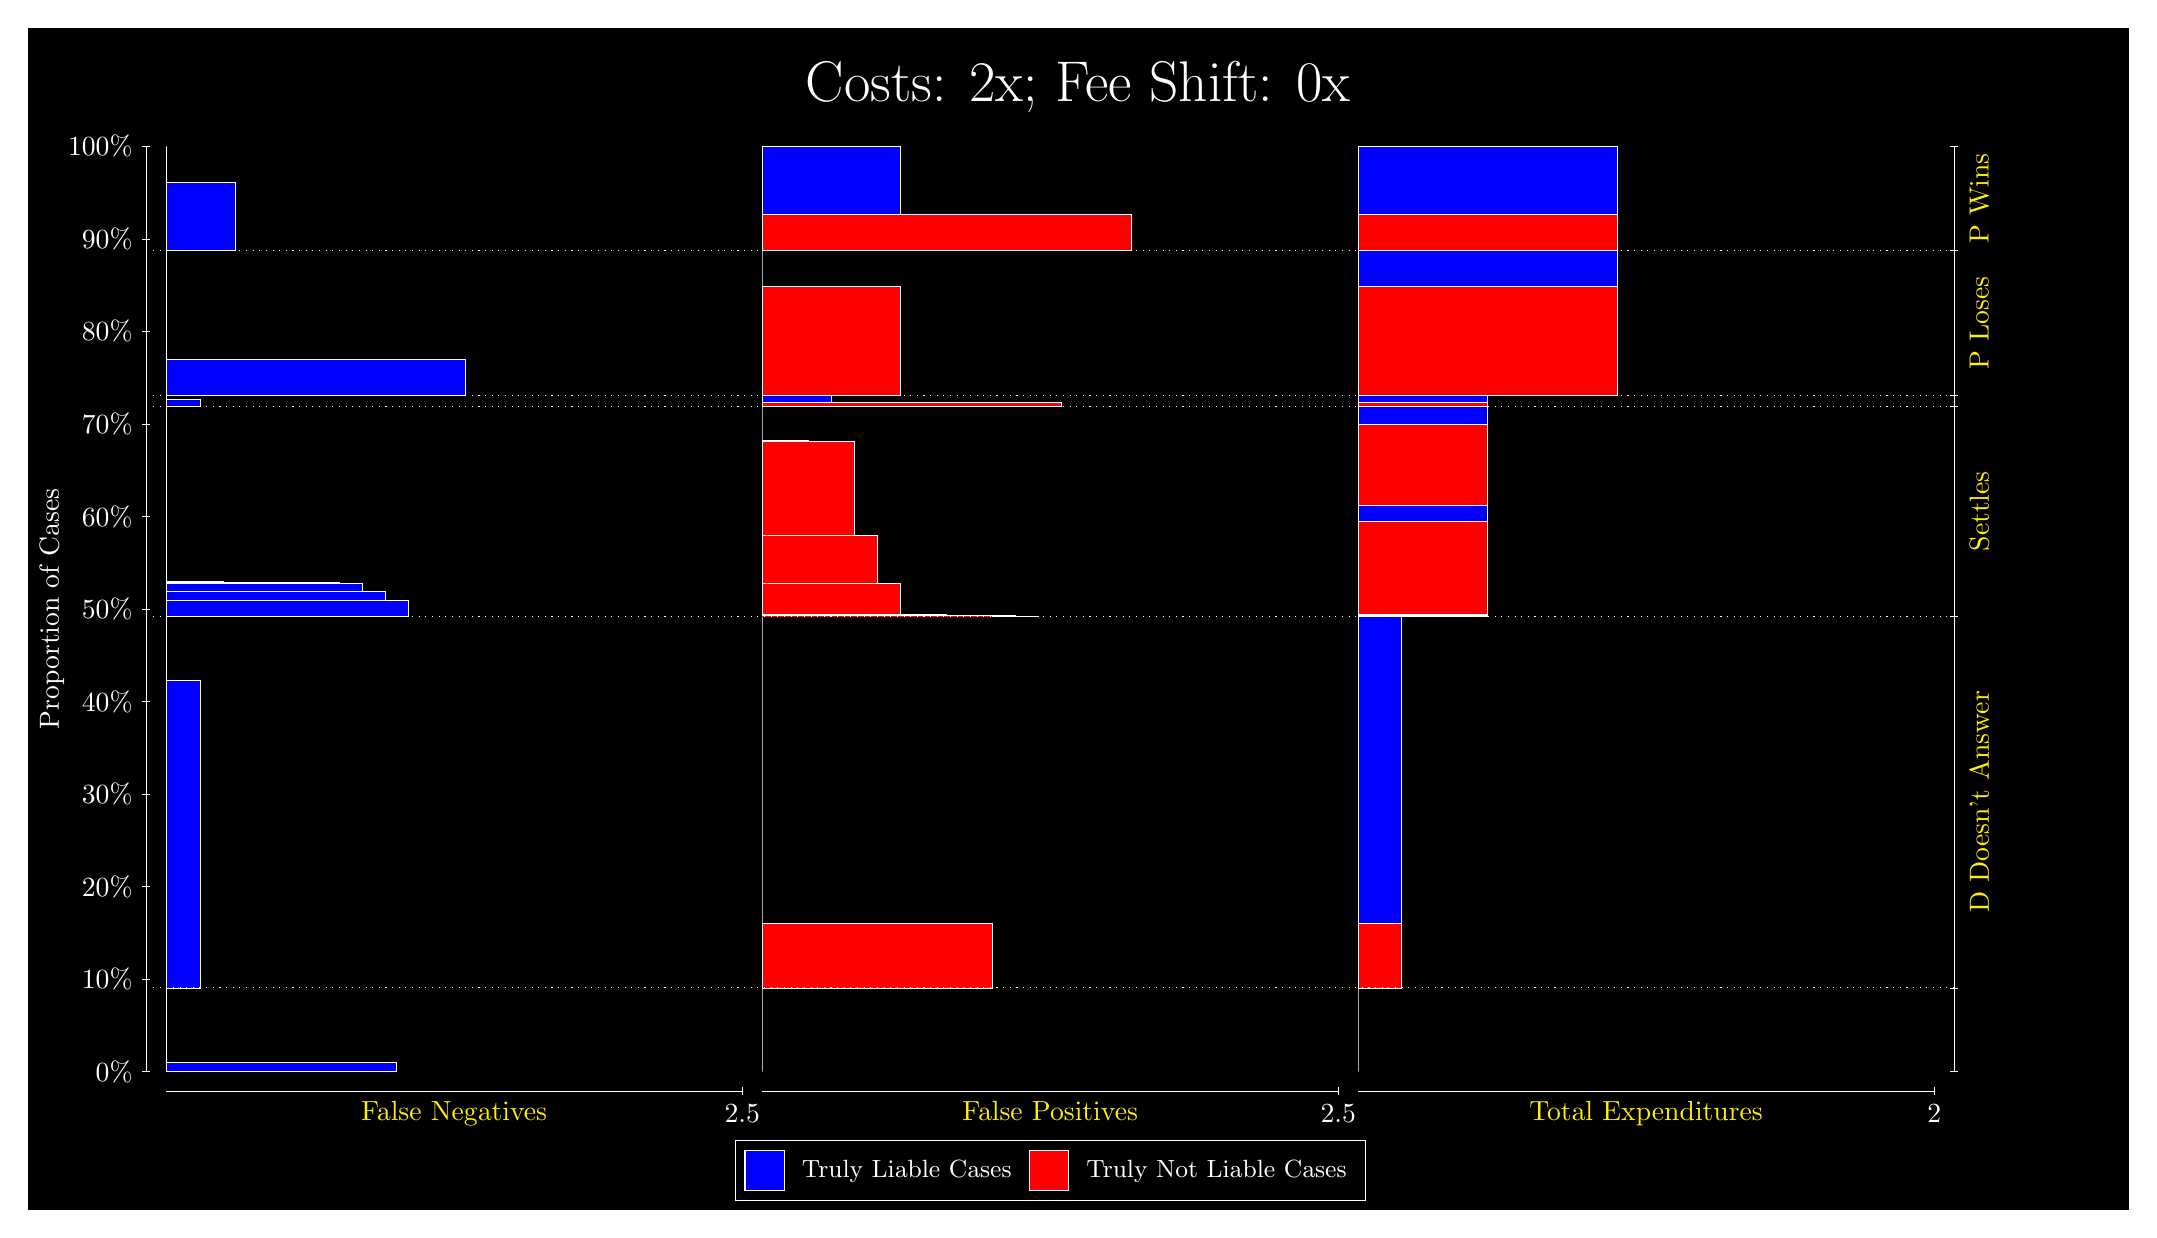
\begin{tikzpicture}
\draw[fill=black] (0,0) rectangle (26.667,15);
\draw[text=white] (0,13.5) rectangle (26.667,15) node[midway] {\huge Costs: 2x; Fee Shift: 0x};
\draw[white, very thin] (1.5,1.75) -- (1.5,13.5);
\node[rotate=90, text=white, anchor=center] at (0.3, 7.625) {Proportion of Cases};
\draw[white, very thin] (1.45,1.75) -- (1.55,1.75);
\node[text=white, anchor=east] at (1.45, 1.75) {0\%};
\draw[white, very thin] (1.45,2.925) -- (1.55,2.925);
\node[text=white, anchor=east] at (1.45, 2.925) {10\%};
\draw[white, very thin] (1.45,4.1) -- (1.55,4.1);
\node[text=white, anchor=east] at (1.45, 4.1) {20\%};
\draw[white, very thin] (1.45,5.275) -- (1.55,5.275);
\node[text=white, anchor=east] at (1.45, 5.275) {30\%};
\draw[white, very thin] (1.45,6.45) -- (1.55,6.45);
\node[text=white, anchor=east] at (1.45, 6.45) {40\%};
\draw[white, very thin] (1.45,7.625) -- (1.55,7.625);
\node[text=white, anchor=east] at (1.45, 7.625) {50\%};
\draw[white, very thin] (1.45,8.8) -- (1.55,8.8);
\node[text=white, anchor=east] at (1.45, 8.8) {60\%};
\draw[white, very thin] (1.45,9.975) -- (1.55,9.975);
\node[text=white, anchor=east] at (1.45, 9.975) {70\%};
\draw[white, very thin] (1.45,11.15) -- (1.55,11.15);
\node[text=white, anchor=east] at (1.45, 11.15) {80\%};
\draw[white, very thin] (1.45,12.325) -- (1.55,12.325);
\node[text=white, anchor=east] at (1.45, 12.325) {90\%};
\draw[white, very thin] (1.45,13.5) -- (1.55,13.5);
\node[text=white, anchor=east] at (1.45, 13.5) {100\%};

\draw[white, very thin] (24.457,1.75) -- (24.457,13.5);
\draw[white, very thin] (24.407,1.75) -- (24.507,1.75);
\node[anchor=west] at (24.407, 1.75) {};
\draw[white, very thin] (24.407,2.8133) -- (24.507,2.8133);
\node[anchor=west] at (24.407, 2.8133) {};
\draw[white, very thin] (24.407,7.5323) -- (24.507,7.5323);
\node[anchor=west] at (24.407, 7.5323) {};
\draw[white, very thin] (24.407,10.199) -- (24.507,10.199);
\node[anchor=west] at (24.407, 10.199) {};
\draw[white, very thin] (24.407,10.334) -- (24.507,10.334);
\node[anchor=west] at (24.407, 10.334) {};
\draw[white, very thin] (24.407,12.177) -- (24.507,12.177);
\node[anchor=west] at (24.407, 12.177) {};
\draw[white, very thin] (24.407,13.5) -- (24.507,13.5);
\node[anchor=west] at (24.407, 13.5) {};

\draw[white, very thin, fill=blue] (1.75,1.75) rectangle (4.6775,1.8619);
\draw[white, very thin, fill=red] (1.75,1.8619) rectangle (1.75,2.8133);
\draw[white, very thin, fill=blue] (1.75,2.8133) rectangle (2.1891,6.7177);
\draw[white, very thin, fill=red] (1.75,6.7177) rectangle (1.75,7.5323);
\draw[white, very thin, fill=blue] (1.75,7.5323) rectangle (4.8239,7.7389);
\draw[white, very thin, fill=blue] (1.75,7.7389) rectangle (4.5312,7.8485);
\draw[white, very thin, fill=blue] (1.75,7.8485) rectangle (4.2384,7.9536);
\draw[white, very thin, fill=blue] (1.75,7.9536) rectangle (3.9457,7.9574);
\draw[white, very thin, fill=blue] (1.75,7.9574) rectangle (3.6529,7.9615);
\draw[white, very thin, fill=blue] (1.75,7.9615) rectangle (3.3602,7.9637);
\draw[white, very thin, fill=blue] (1.75,7.9637) rectangle (3.0674,7.9653);
\draw[white, very thin, fill=blue] (1.75,7.9653) rectangle (2.7746,7.9669);
\draw[white, very thin, fill=blue] (1.75,7.9669) rectangle (2.4819,7.9785);
\draw[white, very thin, fill=red] (1.75,7.9785) rectangle (1.75,10.199);
\draw[white, very thin, fill=blue] (1.75,10.199) rectangle (2.1891,10.286);
\draw[white, very thin, fill=red] (1.75,10.286) rectangle (1.75,10.334);
\draw[white, very thin, fill=blue] (1.75,10.334) rectangle (5.5558,10.793);
\draw[white, very thin, fill=red] (1.75,10.793) rectangle (1.75,12.177);
\draw[white, very thin, fill=blue] (1.75,12.177) rectangle (2.6283,13.043);
\draw[white, very thin, fill=red] (1.75,13.043) rectangle (1.75,13.5);
\draw[white, very thin, fill=red] (9.3189,1.75) rectangle (9.3189,2.7014);
\draw[white, very thin, fill=blue] (9.3189,2.7014) rectangle (9.3189,2.8133);
\draw[white, very thin, fill=red] (9.3189,2.8133) rectangle (12.246,3.6279);
\draw[white, very thin, fill=blue] (9.3189,3.6279) rectangle (9.3189,7.5323);
\draw[white, very thin, fill=red] (9.3189,7.5323) rectangle (12.832,7.5376);
\draw[white, very thin, fill=red] (9.3189,7.5376) rectangle (12.539,7.5392);
\draw[white, very thin, fill=red] (9.3189,7.5392) rectangle (12.246,7.5408);
\draw[white, very thin, fill=red] (9.3189,7.5408) rectangle (11.954,7.5446);
\draw[white, very thin, fill=red] (9.3189,7.5446) rectangle (11.661,7.5533);
\draw[white, very thin, fill=red] (9.3189,7.5533) rectangle (11.368,7.5613);
\draw[white, very thin, fill=red] (9.3189,7.5613) rectangle (11.075,7.9563);
\draw[white, very thin, fill=red] (9.3189,7.9563) rectangle (10.783,8.5662);
\draw[white, very thin, fill=red] (9.3189,8.5662) rectangle (10.49,9.7531);
\draw[white, very thin, fill=blue] (9.3189,9.7531) rectangle (9.9044,9.7647);
\draw[white, very thin, fill=blue] (9.3189,9.7647) rectangle (9.6116,9.7663);
\draw[white, very thin, fill=blue] (9.3189,9.7663) rectangle (9.3189,10.199);
\draw[white, very thin, fill=red] (9.3189,10.199) rectangle (13.125,10.247);
\draw[white, very thin, fill=blue] (9.3189,10.247) rectangle (10.197,10.334);
\draw[white, very thin, fill=red] (9.3189,10.334) rectangle (11.075,11.718);
\draw[white, very thin, fill=blue] (9.3189,11.718) rectangle (9.3189,12.177);
\draw[white, very thin, fill=red] (9.3189,12.177) rectangle (14.003,12.634);
\draw[white, very thin, fill=blue] (9.3189,12.634) rectangle (11.075,13.5);
\draw[white, very thin, fill=red] (16.888,1.75) rectangle (16.888,2.7014);
\draw[white, very thin, fill=blue] (16.888,2.7014) rectangle (16.888,2.8133);
\draw[white, very thin, fill=red] (16.888,2.8133) rectangle (17.437,3.6279);
\draw[white, very thin, fill=blue] (16.888,3.6279) rectangle (17.437,7.5323);
\draw[white, very thin, fill=red] (16.888,7.5323) rectangle (18.534,7.5442);
\draw[white, very thin, fill=blue] (16.888,7.5442) rectangle (18.534,7.5515);
\draw[white, very thin, fill=red] (16.888,7.5515) rectangle (18.534,8.7384);
\draw[white, very thin, fill=blue] (16.888,8.7384) rectangle (18.534,8.945);
\draw[white, very thin, fill=red] (16.888,8.945) rectangle (18.534,9.967);
\draw[white, very thin, fill=blue] (16.888,9.967) rectangle (18.534,10.199);
\draw[white, very thin, fill=red] (16.888,10.199) rectangle (18.534,10.247);
\draw[white, very thin, fill=blue] (16.888,10.247) rectangle (18.534,10.334);
\draw[white, very thin, fill=red] (16.888,10.334) rectangle (20.181,11.718);
\draw[white, very thin, fill=blue] (16.888,11.718) rectangle (20.181,12.177);
\draw[white, very thin, fill=red] (16.888,12.177) rectangle (20.181,12.634);
\draw[white, very thin, fill=blue] (16.888,12.634) rectangle (20.181,13.5);
\draw[white, dotted] (1.5,2.8133) -- (24.457,2.8133);
\draw[white, dotted] (1.5,7.5323) -- (24.457,7.5323);
\draw[white, dotted] (1.5,10.199) -- (24.457,10.199);
\draw[white, dotted] (1.5,10.334) -- (24.457,10.334);
\draw[white, dotted] (1.5,12.177) -- (24.457,12.177);
\draw[white, very thin] (1.75,1.5) -- (9.0689,1.5);
\node[text=yellow, anchor=north] at (5.4094, 1.5) {False Negatives};
\draw[white, very thin] (9.0689,1.45) -- (9.0689,1.55);
\node[text=white, anchor=north] at (9.0689, 1.45) {2.5};

\draw[white, very thin] (9.3189,1.5) -- (16.638,1.5);
\node[text=yellow, anchor=north] at (12.978, 1.5) {False Positives};
\draw[white, very thin] (16.638,1.45) -- (16.638,1.55);
\node[text=white, anchor=north] at (16.638, 1.45) {2.5};

\draw[white, very thin] (16.888,1.5) -- (24.207,1.5);
\node[text=yellow, anchor=north] at (20.547, 1.5) {Total Expenditures};
\draw[white, very thin] (24.207,1.45) -- (24.207,1.55);
\node[text=white, anchor=north] at (24.207, 1.45) {2};


\node[text=yellow, centered, rotate=90] at (24.777, 5.1728) {D Doesn't Answer};
\node[text=yellow, centered, rotate=90] at (24.777, 8.8658) {Settles};

\node[text=yellow, centered, rotate=90] at (24.777, 11.256) {P Loses};
\node[text=yellow, centered, rotate=90] at (24.777, 12.839) {P Wins};

\draw (12.978300999999998,1.5) node[draw=none] (baseCoordinate) {};
\begin{scope}[align=center]
        \matrix[scale=0.5, draw=white, below=0.5cm of baseCoordinate, nodes={draw}, column sep=0.1cm]{
            \node[rectangle, draw, minimum width=0.5cm, minimum height=0.5cm, fill=blue] {}; &
            \node[draw=none, font=\small, text=white] (B) {Truly Liable Cases}; &
            \node[rectangle, draw, minimum width=0.5cm, minimum height=0.5cm, fill=red] {}; &
            \node[draw=none, font=\small, text=white] (B) {Truly Not Liable Cases}; \\
            };
\end{scope}

\end{tikzpicture}
\end{document}